\documentclass{article}
\author{}
\usepackage[utf8]{inputenc}
\usepackage{amsmath}
\usepackage{amssymb}
\usepackage{amsmath,amsthm,amssymb,scrextend}
\usepackage{fancyhdr}
\usepackage{graphicx}
\usepackage{hyperref}

% School name and logo
\newcommand{\schoolname}{Vietnam National University Ho Chi Minh City \\ Ho Chi Minh City University of Technology \\ Faculty of Computer Science and Engineering}
\newcommand{\schoollogo}{
\includegraphics[width=3cm]{img/hcmut.png}}

\begin{document}
\begin{titlepage}
    \centering
    \vspace*{2cm}
    \schoollogo\par
    \vspace{1cm}
    {\Large \schoolname\par}
    \vspace{3cm}
    {\huge\bfseries Internship I -\ Report \par}
    \vspace{1cm}
    {\Large\bfseries Supervisor: Assoc. Prof.\ Quan Thanh Tho \par}
    \vspace{1cm}
    {\large \bfseries Tang Quoc Thai -\ 2270376\par}
    \vfill
    {\large \today\par}
\end{titlepage}

\section{Motivation}
\section{Theoretical Background}
\subsection{Phoneme Segmentation}
\begin{sloppypar}
Detecting phoneme boundaries or segmenting phonemes is a crucial initial step in various speech processing applications, including speaker diarization~\cite{moattar2012review}, speech science~\cite{adi2016automatic, adi2015vowel}, keyword spotting~\cite{keshet2009discriminative}, Automatic Speech Recognition~\cite{kubala1996transcribing, rybach2009audio}, and more. These segmentations are typically achieved through supervised or unsupervised methods. In the unsupervised approach, only the speech signal is used as input~\cite{michel2016blind, sorin2006relation}, while in the supervised approach, the speech signal is accompanied by target boundaries for guidance. In supervised scenarios, the set of pronounced or presumed phonemes is often provided as additional input, known as forced alignment. When no phonemes are supplied, the setup is termed text-independent phoneme segmentation~\cite{aversano2001new, chen2016text}. This study specifically focuses on the supervised text-independent phoneme segmentation problem.\\[5mm]
\begin{figure}[htbp]
    \centering
    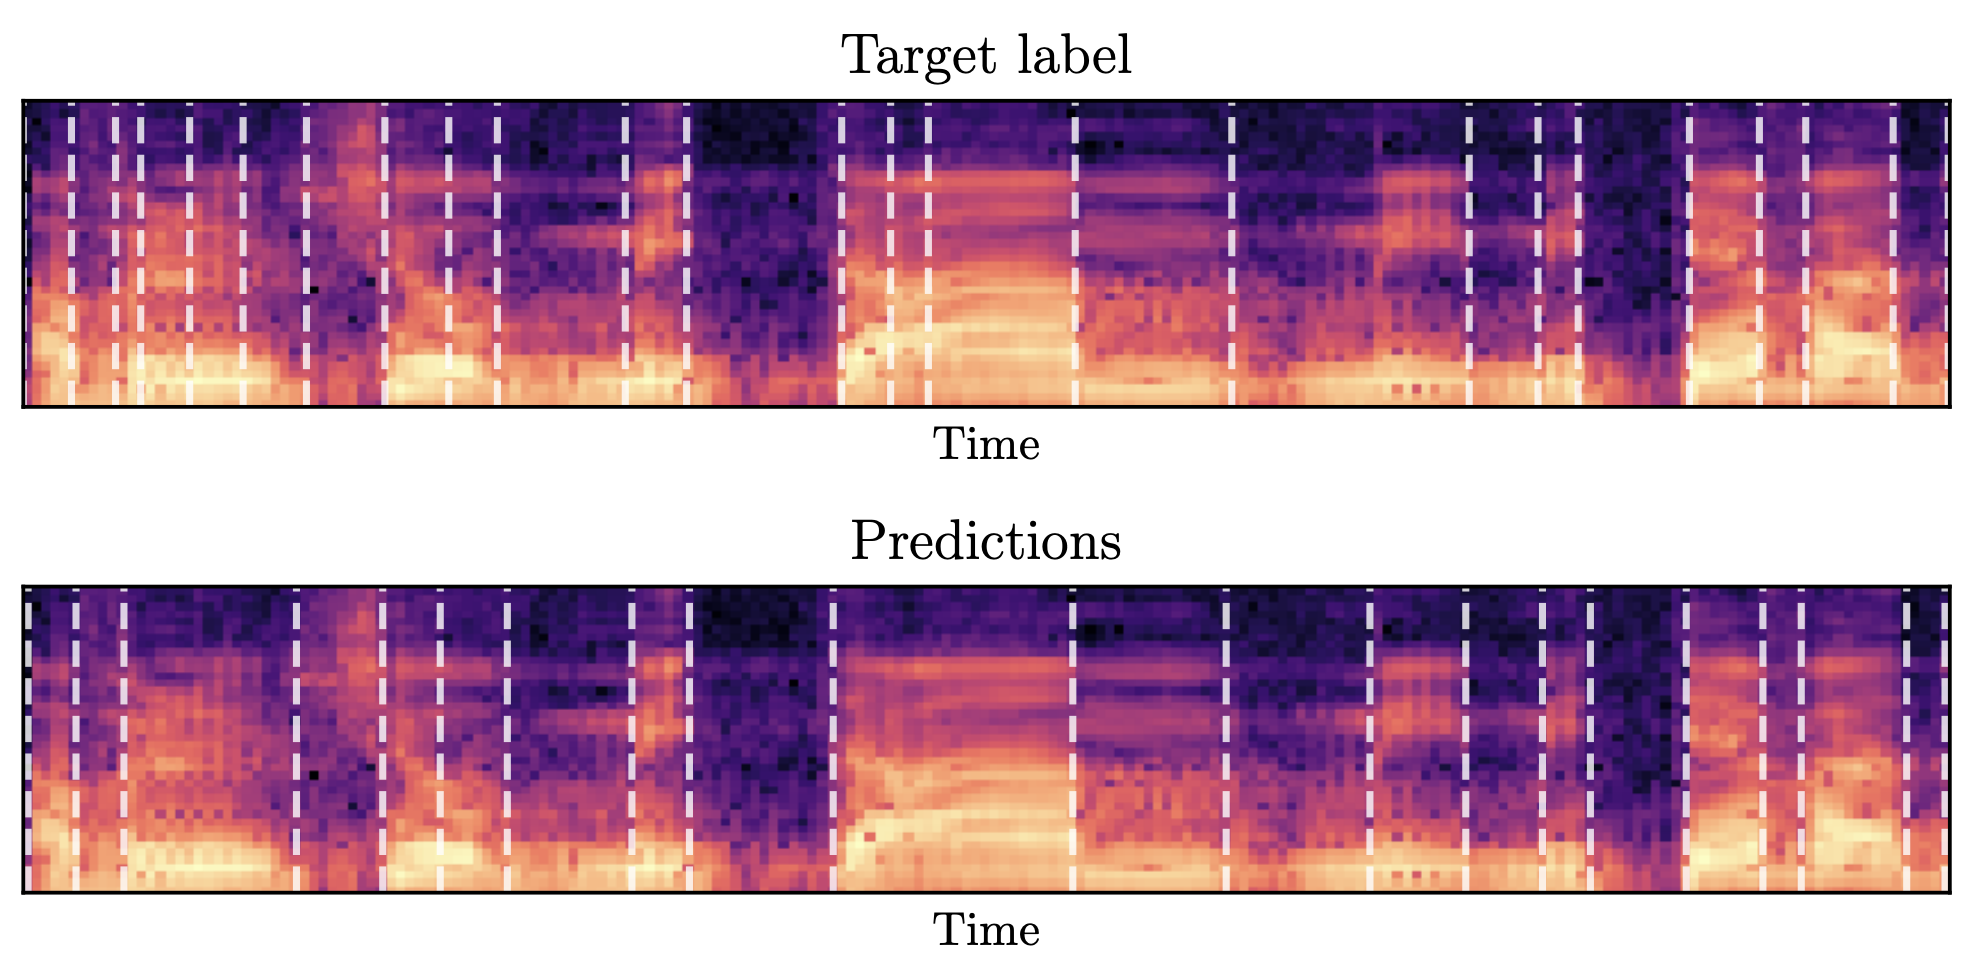
\includegraphics[width=0.8\textwidth]{img/phoneme_boundary_detection.png}
    \caption{Example of supervised phoneme boundary detection.}
\end{figure}
\end{sloppypar}
\subsection{Related Works}
\begin{sloppypar}
Researchers have delved into the challenge of detecting phoneme boundaries across different scenarios. In the unsupervised setting, also termed blind phoneme segmentation, the speech signal is presented without any additional phonemes or boundaries for guidance. Traditionally, signal processing techniques were utilized to identify spectral changes in the signal for phoneme boundary detection~\cite{dusan2006relation, estevan2007finding, hoang2015blind, almpanidis2008phonemic, rasanen2011blind}, as mentioned in the respective references. A recent proposal in~\cite{michel2016blind} suggests training a next-frame prediction model using an approximated Markov model or RNN to pinpoint potential phoneme transitions in regions of high error.\\[5mm]
In the supervised setting, the forced alignment approach is prevalent. Models employing this approach typically involve Hidden Markov Models or various structured prediction algorithms with handcrafted features~\cite{keshet2005phoneme, mcauliffe2017montreal}. However, a significant drawback of forced alignment methods is the necessity for phoneme annotations even during inference, limiting their applicability to monolingual settings due to potential mismatches in phoneme sets from foreign languages.\\[5mm]
Another supervised setting is text-independent phoneme boundary detection, where the model receives phoneme boundaries as supervision but lacks information about the uttered phonemes. In previous works following this setup, the problem is often treated as a binary classification task, associating one label with phoneme boundary annotations and another with the remaining signal. For instance, in~\cite{king2013accurate}, a kernel-based method consisting of six radial basis function support vector machines was employed, while~\cite{franke2016phoneme} suggested using an RNN followed by a peak detection algorithm for predicting phoneme boundaries. However, a drawback of such modeling is the neglect of the internal structure of the output, treating boundaries as conditionally independent.\\[5mm]
Additionally, noteworthy are related lines of work in the domain of learnable segmental features in ASR~\cite{lu2016segmental}, dependency parsing~\cite{kiperwasser2016simple}, and word segmentation~\cite{adi2017sequence}.
\end{sloppypar}
\section{Proposed Method}
\subsection{Data Preprocessing}
\subsection{Feature Extraction}
\section{Experiments}
\section{Conclusion}
\section{References}
\bibliography{references}
\bibliographystyle{unsrt}

\end{document}
